\section{The Gradient}
\noindent
If you are on a surface $f: \mathbb{R}^2 \to \mathbb{R}$, what direction $\langle \Delta x, \Delta y \rangle$ should you go to maximize the change of $f$?\\
We saw earlier that $\Delta z\approx \langle f_x, f_y \rangle \cdot \langle \Delta x, \Delta y \rangle$.
To maximize a dot product, $\langle \Delta x, \Delta y \rangle$ should be in the same direction as $\langle f_x, f_y \rangle$.
This directional vector is called the gradient: the direction of steepest ascent.\\
Notated mathematically,
\begin{equation*}
	\nabla f(x,y) = \langle f_x, f_y \rangle.
\end{equation*}

\begin{figure}[H]
	\centering
	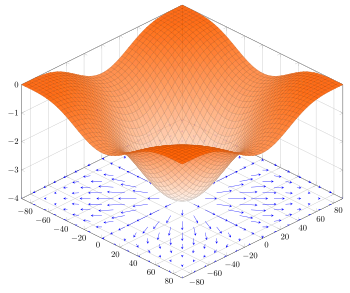
\includegraphics[width=0.5\textwidth]{./differentialMultivariableCalculus/gradient.png}
	\caption{A surface and its gradient vectors}
\end{figure}

\input{./differentialMultivariableCalculus/gradientProperties}
\input{./differentialMultivariableCalculus/linearApproximationsGradient}
\subsection{The Gradient \& C-Level Curves}
\noindent
Let $\vec{r}(t)$ be the C-level curve of $f(x, y)$.
\begin{align*}
f\circ\vec{r} &= C  \text{ and } \frac{\mathrm{d}}{\mathrm{d}t}(f\circ\vec{r}) = 0 \\
	&\implies \frac{\mathrm{d}}{\mathrm{d}t}(f\circ\vec{r}) = \nabla f\cdot\vec{r^\prime}(t) = 0 \\
	&\implies \nabla f\perp\vec{r^\prime}(t) \\
	&\implies \nabla f \text{ is perpendicular to the C-level curve of } f.
\end{align*}

\begin{figure}[H]
	\centering
	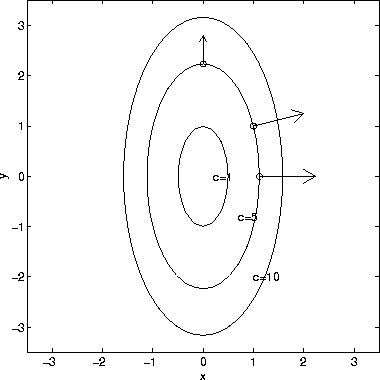
\includegraphics[width=0.33\textwidth]{./differentialMultivariableCalculus/grad_c_level.png}
	\caption{The gradient is perpendicular to C-level curves.}
\end{figure}